\chapter{Mengenali Zat}\label{ch:g7:identifying-substances}

Secarik catatan kusut, ditulis dengan spidol hitam, ditemukan di tempat
sebuah misteri kecil, dan tiga spidol ditemukan di tiga tas yang
berbeda. Di mata kita, ketiga tinta itu tampak sama hitamnya. Seorang
ahli kimia forensik hanya memerlukan secarik kertas, sedikit air, dan
setengah jam untuk mengatakan spidol mana yang menulis catatan itu. Ahli
kimia mengenali zat bukan dari penampilannya, melainkan dari
perilakunya dalam uji yang dipilih khusus untuknya.

\begin{recall}
\omterm{def:g6:pure-substances-and-mixtures:species}{Spesies kimia} adalah satu jenis zat tertentu; \omterm{def:g6:pure-substances-and-mixtures:pure-substance}{zat murni} mengandung satu
spesies saja, \omterm{def:g6:pure-substances-and-mixtures:mixture}{campuran} beberapa spesies
(\cref{ch:g6:pure-substances-and-mixtures}). Ada zat yang mudah \omterm{def:g2:mixing-and-dissolving:dissolve}{larut}
dalam suatu \omterm{def:g6:solutions-and-solubility:solute}{pelarut}, ada pula yang sedikit atau sama sekali tidak \omterm{def:g2:mixing-and-dissolving:dissolve}{larut}:
setiap zat memiliki \omterm{def:g6:solutions-and-solubility:solubility}{kelarutannya} sendiri
(\cref{ch:g6:solutions-and-solubility}).
\end{recall}

\section{Apa itu uji khas}

\begin{definition}[Uji khas dan reagen]\label{def:g7:identifying-substances:characteristic-test}
Sebuah \emph{uji khas}\index{uji khas} untuk suatu \omterm{def:g6:pure-substances-and-mixtures:species}{spesies kimia}
adalah percobaan sederhana yang memberikan hasil yang terlihat dengan
spesies itu, dan tidak dengan spesies lain yang dijumpai dalam situasi
yang sama. Uji itu memakai zat yang dipilih untuk keperluan tersebut,
yaitu \emph{reagen}\index{reagen}.
\end{definition}


\begin{method}[Melakukan uji khas]\label{met:g7:identifying-substances:run}
\begin{enumerate}
  \item Ambil sedikit sampel zat yang akan diuji.
  \item Tambahkan \omterm{def:g7:identifying-substances:characteristic-test}{reagennya}, atau sentuhkan \omterm{def:g7:identifying-substances:characteristic-test}{reagen} itu dengan sampel,
        seperti yang diuraikan dalam uji.
  \item Amati: perubahan warna, kekeruhan, nyala api, bunyi.
  \item Simpulkan: uji itu \emph{positif} jika hasil yang diharapkan
        muncul, \emph{negatif} jika tidak.
  \item Lakukan uji yang sama pada sampel yang diketahui tidak
        mengandung spesies itu (blanko): hasilnya harus tetap negatif,
        kalau tidak, hasil uji itu tidak membuktikan apa pun.
\end{enumerate}
\end{method}

\section{Empat uji klasik}

\begin{proposition}[Karbon dioksida mengeruhkan air kapur]\label{prop:g7:identifying-substances:limewater}
Air kapur adalah larutan yang jernih dan tak berwarna. Jika karbon
dioksida dialirkan ke dalamnya, air kapur menjadi keruh seputih susu.
\omterm{def:g4:air-a-mixture-of-gases:air}{Udara} yang diembuskan melalui sedotan mengeruhkan air kapur; \omterm{def:g4:air-a-mixture-of-gases:air}{udara}
segar yang dipompakan ke dalamnya hampir tidak mengeruhkannya.
\end{proposition}

\begin{omfigure}
\begin{tikzpicture}[font=\small, scale=1.25]
  % generating tube, stoppered
  \pic[transform shape] at (0,0) {testtube={0.35}{omWater!80}};
  \fill[black!65] (-0.27,2.8) rectangle (0.27,3.15);
  \foreach \y in {0.4,0.65,0.85} \draw[black!55] (0.05,\y) circle (0.04);
  \pic[transform shape] at (0,2.9) {deliverytube={1.9}{-2.3}};
  % limewater tube
  \pic[transform shape] at (1.9,0) {testtube={0.6}{white!85!black}};
  \foreach \x/\y in {1.88/0.75,1.95/1.0,1.85/1.25,1.92/1.5} \draw[black!55] (\x,\y) circle (0.04);
  \draw[<-, omProp, thick] (-0.3,0.5) -- (-1.2,0.8) node[left, text=black, align=right]
    {reaksi yang\\ melepaskan gas};
  \draw[<-, omProp, thick] (2.2,1.2) -- (3.0,1.4) node[right, text=black, align=left]
    {air kapur menjadi\\ keruh: gas itu\\ karbon dioksida};
\end{tikzpicture}

{\small Uji air kapur. Gas yang dilepaskan di tabung pertama dialirkan
melalui air kapur; jika air kapur menjadi keruh, gas itu adalah karbon
dioksida.}
\end{omfigure}

\begin{proposition}[Air membirukan tembaga sulfat anhidrat]\label{prop:g7:identifying-substances:copper-sulfate}
Tembaga sulfat anhidrat adalah serbuk putih. Setetes air langsung
membuatnya biru. Uji ini menunjukkan adanya air, dalam cairan atau dalam
padatan yang lembap --- bukan bahwa cairan itu air murni.
\end{proposition}

\begin{omfigure}
\begin{minipage}[b]{0.48\linewidth}\centering
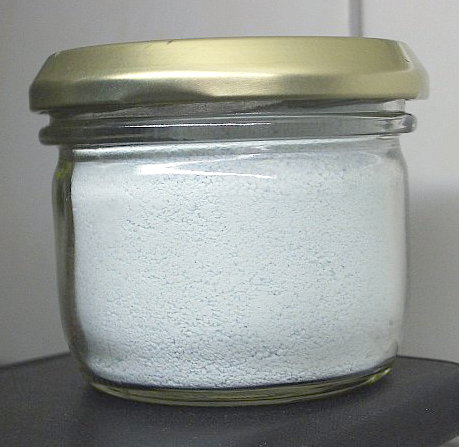
\includegraphics[width=\linewidth,height=4.2cm,keepaspectratio]{images/book1/cuso4-anhydrous.jpg}

{\small Tembaga sulfat anhidrat: serbuk putih. Foto: W.~Oelen,
CC\ BY-SA\ 3.0.}
\end{minipage}\hfill
\begin{minipage}[b]{0.48\linewidth}\centering
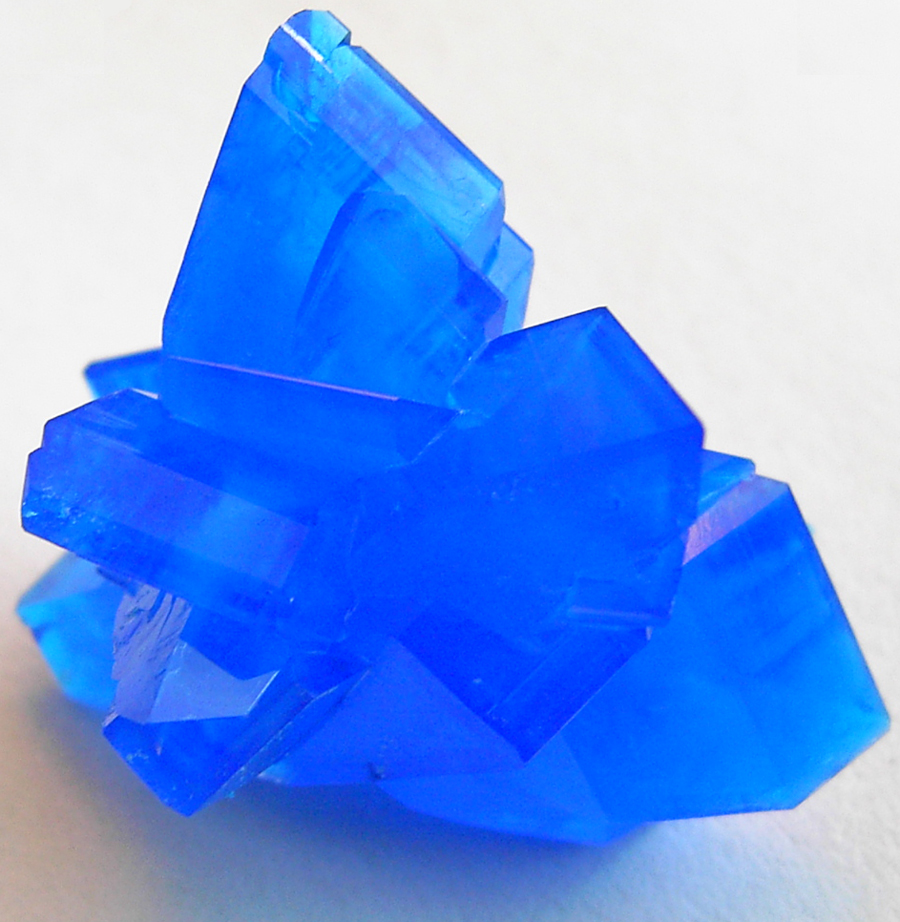
\includegraphics[width=\linewidth,height=4.2cm,keepaspectratio]{images/book1/cuso4-hydrated.jpg}

{\small Dengan air, serbuk itu menjadi biru; kristal-kristal ini
mengandung air. Foto: Stephanb, CC\ BY-SA\ 3.0.}
\end{minipage}
\end{omfigure}

\begin{safety}{\ghs[0.82cm]{GHS05}\ghs[0.82cm]{GHS07}\ghs[0.82cm]{GHS09}}
% ledger: ghs:CuSO4
Tembaga sulfat: berbahaya jika tertelan dan menyebabkan iritasi kulit
(GHS07); dapat merusak mata secara serius (GHS05); sangat beracun bagi
kehidupan akuatik, dengan dampak jangka panjang (GHS09). Pakai kacamata
pelindung dan sarung tangan; limbahnya dikumpulkan, tidak pernah
dibuang ke bak cuci.
\end{safety}

\begin{proposition}[Oksigen menyalakan kembali bilah kayu yang berbara]\label{prop:g7:identifying-substances:splint}
Sebatang bilah kayu dinyalakan, lalu ditiup padam sehingga hanya bara
merahnya yang tersisa. Jika dimasukkan ke dalam tabung reaksi berisi
oksigen, bilah kayu yang berbara itu menyala kembali.
\end{proposition}

\begin{proposition}[Hidrogen terbakar dengan letupan melengking]\label{prop:g7:identifying-substances:pop}
Bilah kayu menyala yang didekatkan ke mulut tabung reaksi kecil berisi
hidrogen menimbulkan bunyi ``pop'' yang pendek dan melengking: hidrogen
langsung \omterm{def:g4:what-a-fire-needs:burning}{terbakar} bersama oksigen dari \omterm{def:g4:air-a-mixture-of-gases:air}{udara}.
\end{proposition}

\begin{omfigure}
\begin{tikzpicture}[font=\small, scale=1.25]
  % splint test for oxygen
  \pic[transform shape] at (0,0) {testtube={0}{white}};
  \draw[brown!60!black, line width=2pt] (0.15,1.6) -- (1.4,3.6);
  \fill[orange!85] (0.15,1.6) circle (0.07);
  \fill[orange!80] (0.12,1.62) .. controls (0.0,1.9) and (0.08,2.1) .. (0.1,2.3)
    .. controls (0.2,2.05) and (0.3,1.85) .. (0.2,1.62);
  \node[anchor=north, align=center] at (0,-0.15) {oksigen:\\ bilah yang berbara\\ menyala kembali};
  % pop test for hydrogen
  \begin{scope}[xshift=4cm]
    \pic[transform shape, rotate=180] at (0,3.1) {testtube={0}{white}};
    \draw[brown!60!black, line width=2pt] (0.05,-0.05) -- (1.3,-0.9);
    \fill[orange!85] (0.05,-0.02) .. controls (-0.05,0.08) and (0.0,0.15) .. (0.02,0.22)
      .. controls (0.08,0.15) and (0.15,0.08) .. (0.1,-0.02);
    \node[font=\small\itshape] at (-0.9,0.15) {pop!};
    \node[anchor=north, align=center] at (0,-1.0) {hidrogen:\\ letupan melengking\\ di mulut tabung};
  \end{scope}
\end{tikzpicture}

{\small Kiri: bilah kayu berbara menyala kembali di dalam oksigen. Kanan:
bilah kayu menyala di mulut tabung hidrogen yang terbalik menimbulkan
letupan melengking (hidrogen lebih ringan daripada \omterm{def:g4:air-a-mixture-of-gases:air}{udara}, jadi mulut
tabungnya dihadapkan ke bawah).}
\end{omfigure}

\begin{safety}{\ghs[0.82cm]{GHS02}\ghs[0.82cm]{GHS04}}
% ledger: ghs:H2
Hidrogen: gas yang sangat mudah menyala (GHS02), disimpan di bawah
tekanan dalam tabung (GHS04). Uji letupan dilakukan hanya dengan
beberapa mililiter, oleh guru.
\end{safety}

\section{Kromatografi kertas}

\begin{definition}[Kromatografi kertas dan kromatogram]\label{def:g7:identifying-substances:chromatography}
Yang disebut \emph{kromatografi kertas}\index{kromatografi kertas} adalah
cara memisahkan zat-zat warna sebuah \omterm{def:g6:pure-substances-and-mixtures:mixture}{campuran}. Setitik kecil \omterm{def:g6:pure-substances-and-mixtures:mixture}{campuran}
diletakkan pada garis yang digambar di dekat bagian bawah secarik
kertas; ujung bawah kertas itu dicelupkan ke dalam \omterm{def:g6:solutions-and-solubility:solute}{pelarut}, yang
perlahan naik melalui kertas dan membawa setiap zat warna bersamanya,
ada yang lebih cepat daripada yang lain. Ketika \omterm{def:g6:solutions-and-solubility:solute}{pelarut} sudah naik
hampir sampai ke atas, kertas itu diangkat dan dikeringkan: inilah
\emph{kromatogram}\index{kromatogram}.
\end{definition}

\begin{omfigure}
\begin{tikzpicture}[font=\small, scale=1.3]
  % the strip in a beaker of solvent
  \pic[transform shape] at (0,0) {beaker={0.12}{omWater!80}};
  \fill[white] (-0.42,0.06) rectangle (0.42,2.2);
  \fill[omWater!80] (-0.42,0.06) rectangle (0.42,0.24);
  \draw[omGlass, line width=0.6pt] (-0.42,0.06) rectangle (0.42,2.2);
  \draw[black!60, line width=0.4pt] (-0.42,0.42) -- (0.42,0.42);
  \fill[black!80] (0,0.42) circle (0.07);
  \shade[ball color=black!20] (0,2.27) circle (0.08);
  \draw[black!50, line width=1.2pt] (-1.1,2.27) -- (1.1,2.27);
  \node[anchor=north, align=center] at (0,-0.15) {pada awalnya};
  \draw[<-, omProp, thick] (0.1,0.5) -- (1.3,0.8) node[right, text=black]
    {titik tinta pada garis pensil};
  \draw[<-, omProp, thick] (1.0,2.27) -- (1.3,2.5) node[right, text=black]
    {batang kaca penahan kertas};
  \draw[<-, omProp, thick] (0.75,0.15) -- (1.3,0.25) node[right, text=black]
    {pelarut, di bawah garis};
  % the chromatogram
  \begin{scope}[xshift=6.2cm]
    \pic[transform shape] at (0,0) {tlcplate};
    \draw[black!50, dashed] (-0.7,2.7) -- (0.7,2.7);
    \fill[blue!70] (0,1.0) ellipse (0.13 and 0.09);
    \fill[red!70] (0,1.7) ellipse (0.13 and 0.09);
    \fill[yellow!80!orange] (0,2.35) ellipse (0.13 and 0.09);
    \node[anchor=north, align=center] at (0,-0.15) {kromatogramnya};
    \draw[<-, omProp, thick] (0.75,2.7) -- (1.3,2.85) node[right, text=black]
      {batas naik pelarut};
    \draw[<-, omProp, thick] (0.2,1.7) -- (1.3,1.7) node[right, text=black]
      {tiga zat warna: campuran};
  \end{scope}
\end{tikzpicture}

{\small \omterm{def:g7:identifying-substances:chromatography}{Kromatografi kertas} tinta hitam. \omterm{def:g6:solutions-and-solubility:solute}{Pelarut} naik melalui kertas dan
memisahkan tinta itu menjadi tiga zat warna.}
\end{omfigure}

\begin{method}[Membaca kromatogram]\label{met:g7:identifying-substances:read}
\begin{enumerate}
  \item Hitung bercak di atas setiap titik awal: satu bercak, satu zat
        warna; dua bercak atau lebih, \omterm{def:g6:pure-substances-and-mixtures:mixture}{campuran} zat warna.
  \item Bandingkan tingginya: pada \omterm{def:g7:identifying-substances:chromatography}{kromatogram} yang sama, satu zat warna
        selalu naik sampai ketinggian yang sama. Bercak yang setinggi zat
        warna yang sudah diketahui kemungkinan besar adalah zat warna itu.
  \item Pakailah garis pensil, jangan tinta: tinta itu sendiri akan
        dipisahkan oleh \omterm{def:g6:solutions-and-solubility:solute}{pelarut}.
\end{enumerate}
\end{method}

\begin{example}[Zat warna permen]\label{ex:g7:identifying-substances:sweets}
Lapisan berwarna pada permen dikerok ke dalam sedikit air lalu
ditotolkan pada secarik kertas, di samping totolan zat-zat warna makanan
yang diizinkan untuk permen. \omterm{def:g7:identifying-substances:chromatography}{Kromatogramnya} menunjukkan bahwa lapisan
hijau mengandung satu zat warna kuning dan satu zat warna biru, keduanya
termasuk zat warna yang diizinkan.
\end{example}


\section{Membaca bank uji}

\begin{proposition}[Tabel uji khas]\label{prop:g7:identifying-substances:bank}
Para ahli kimia menyimpan uji-uji yang mereka pakai dalam sebuah tabel,
bank uji, yang dibaca dari kiri ke kanan:
\begin{center}
\small
\begin{tabular}{llll}
\hline
spesies yang dicari & \omterm{def:g7:identifying-substances:characteristic-test}{reagen} atau uji & hasil positif & \\
\hline
karbon dioksida & air kapur & air kapur menjadi keruh & \\
air & tembaga sulfat anhidrat & putih menjadi biru & \\
oksigen & bilah kayu berbara & bilah menyala kembali & \\
hidrogen & bilah kayu menyala & letupan melengking & \\
zat warna \omterm{def:g6:pure-substances-and-mixtures:mixture}{campuran} & \omterm{def:g7:identifying-substances:chromatography}{kromatografi kertas} & satu bercak per zat warna & \\
\hline
\end{tabular}
\end{center}
\end{proposition}

\begin{remark}[Yang tidak dikatakan oleh sebuah uji]\label{rem:g7:identifying-substances:limits}
Uji yang positif membuktikan bahwa spesies itu ada, bukan bahwa spesies
itu sendirian: cairan yang membirukan tembaga sulfat mengandung air,
tetapi cairan itu mungkin air asin atau jus jeruk. Uji yang negatif
hanya mengatakan bahwa spesies itu tidak ada, atau ada dalam jumlah yang
terlalu kecil untuk terlihat.
\end{remark}

\begin{omfigure}
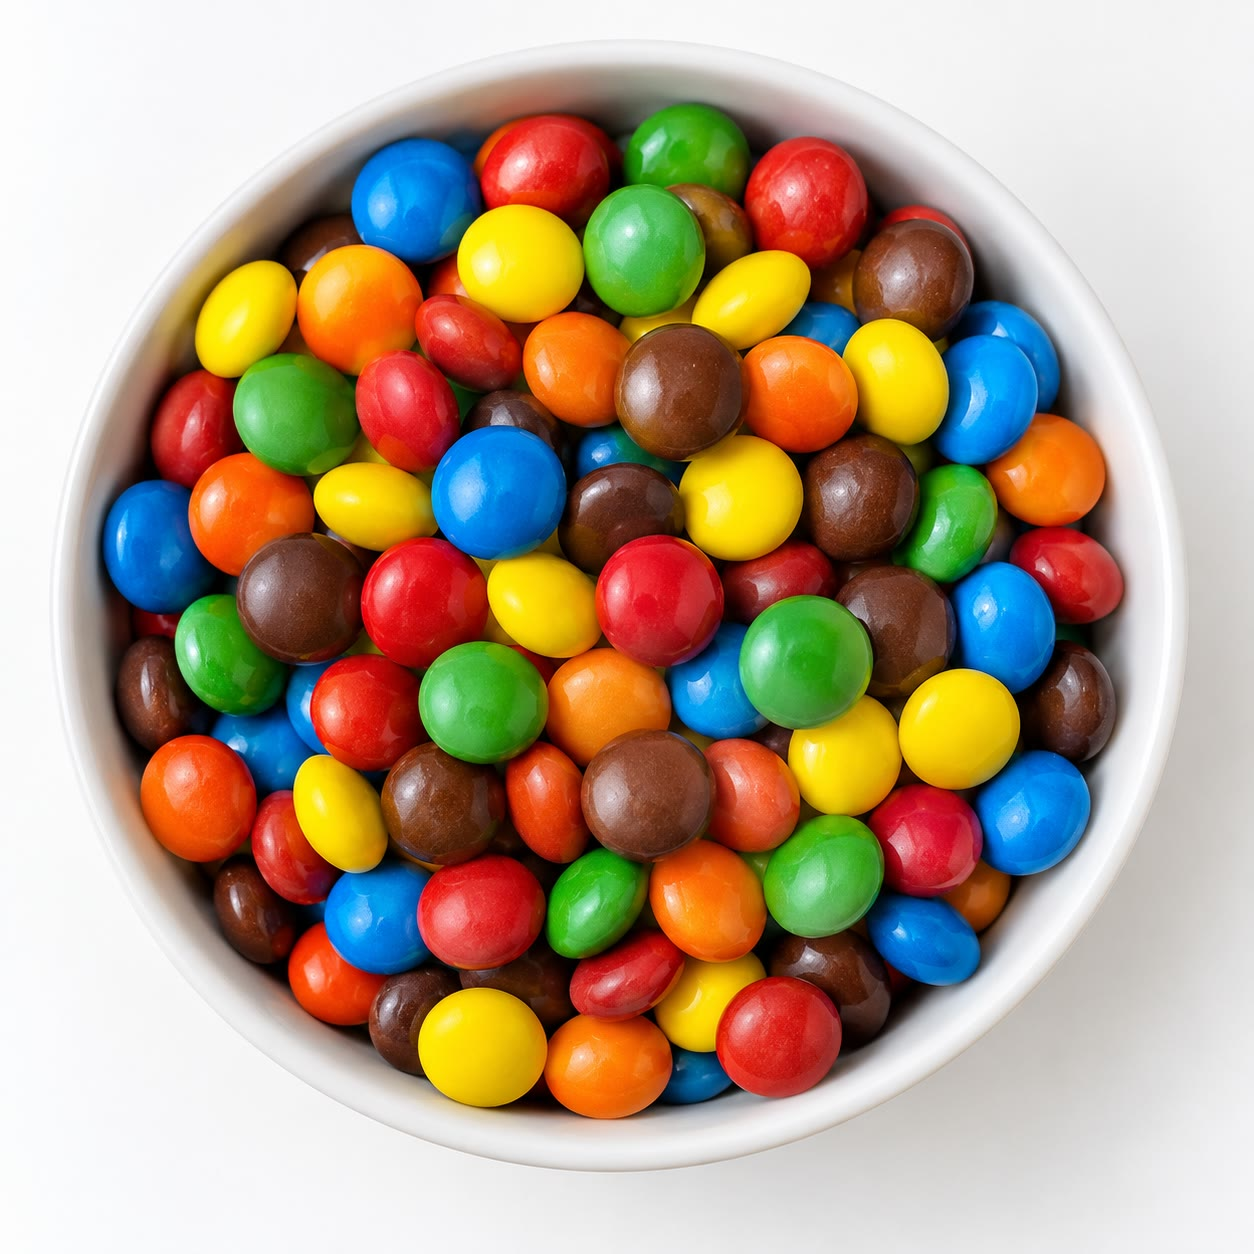
\includegraphics[width=0.32\linewidth]{images/book1/ai/g7-sweets.jpg}

{\small Permen berlapis gula: warnanya adalah \omterm{def:g6:pure-substances-and-mixtures:mixture}{campuran} zat warna yang
dapat dipisahkan dengan kromatografi.}
\end{omfigure}

\begin{omfigure}
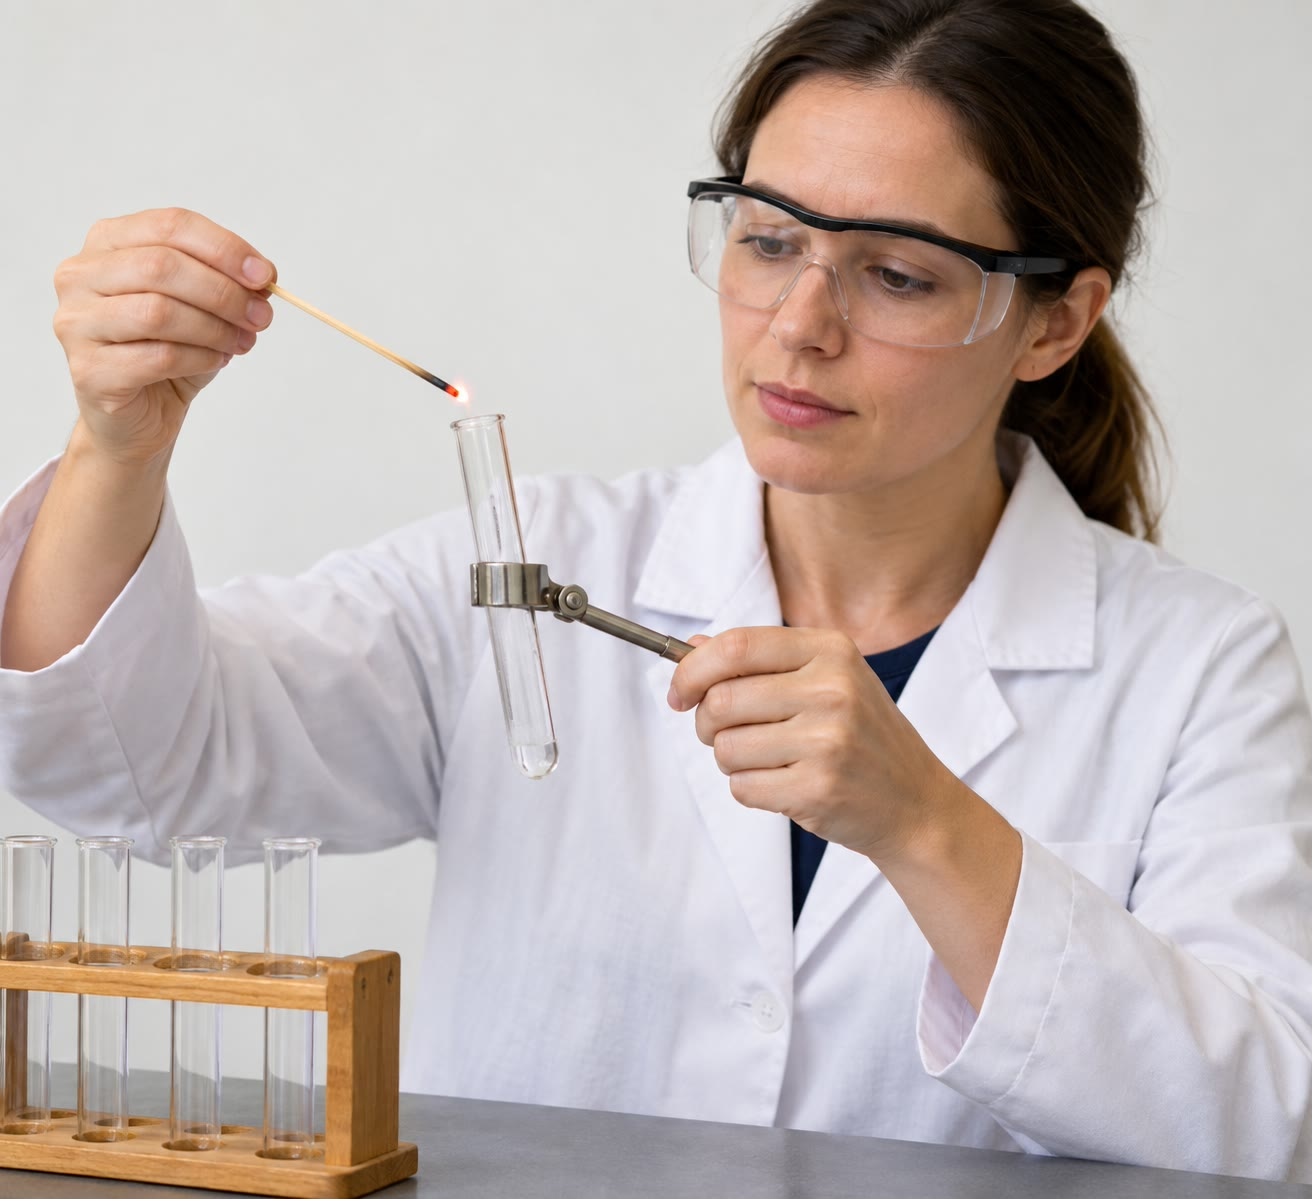
\includegraphics[width=0.36\linewidth]{images/book1/ai/g7-splint-teacher.jpg}

{\small Seorang guru menguji gas dengan bilah kayu yang berbara.}
\end{omfigure}

\section{Latihan}

\begin{exercise}[$\star$]\label{exo:g7:identifying-substances:1}
Uji apa yang mengenali karbon dioksida? Uraikan hasil positifnya.
\end{exercise}

\begin{exercise}[$\star$]\label{exo:g7:identifying-substances:2}
Serbuk putih menjadi biru ketika sebuah cairan diteteskan ke atasnya.
Apa yang ditunjukkan hal ini tentang cairan itu?
\end{exercise}

\begin{exercise}[$\star$]\label{exo:g7:identifying-substances:3}
Bilah kayu berbara dimasukkan ke dalam tabung gas dan menyala kembali.
Gas apa yang ada di dalam tabung itu?
\end{exercise}

\begin{exercise}[$\star$]\label{exo:g7:identifying-substances:4}
Mengapa garis awal \omterm{def:g7:identifying-substances:chromatography}{kromatogram} kertas digambar dengan pensil dan bukan
dengan tinta?
\end{exercise}

\begin{exercise}[$\star\star$]\label{exo:g7:identifying-substances:5}
Mengapa garis awal harus berada di atas permukaan \omterm{def:g6:solutions-and-solubility:solute}{pelarut} di dalam
gelas kimia?
\end{exercise}

\begin{exercise}[$\star\star$]\label{exo:g7:identifying-substances:6}
\omterm{def:g7:identifying-substances:chromatography}{Kromatogram} tinta hijau memperlihatkan dua bercak, satu setinggi zat
warna kuning pembanding, satu setinggi zat warna biru pembanding.
Apakah tinta hijau itu \omterm{def:g6:pure-substances-and-mixtures:pure-substance}{zat murni}? Terbuat dari apakah tinta itu?
\end{exercise}

\begin{exercise}[$\star\star$]\label{exo:g7:identifying-substances:7}
Dengan bank uji, uji apa yang akan kamu pakai untuk menunjukkan bahwa
gas yang dilepaskan sebuah reaksi adalah hidrogen? Apa yang kamu
harapkan terlihat?
\end{exercise}

\begin{exercise}[$\star\star$]\label{exo:g7:identifying-substances:8}
\omterm{def:g4:air-a-mixture-of-gases:air}{Udara} yang diembuskan mengeruhkan air kapur jauh lebih cepat daripada
\omterm{def:g4:air-a-mixture-of-gases:air}{udara} segar. Apa yang ditunjukkan hal ini tentang \omterm{def:g4:air-a-mixture-of-gases:air}{udara} yang kita
embuskan?
\end{exercise}

\begin{exercise}[$\star\star$]\label{exo:g7:identifying-substances:9}
Sebuah cairan jernih membirukan tembaga sulfat anhidrat. Sam
menyimpulkan: ``Itu air murni.'' Jelaskan mengapa Sam keliru.
\end{exercise}

\begin{exercise}[$\star\star$]\label{exo:g7:identifying-substances:10}
Lihatlah \omterm{def:g7:identifying-substances:chromatography}{kromatogram} tinta hitam dalam bab ini. Berapa zat warna yang
dikandung tinta itu? Zat warna mana yang naik paling tinggi?
\end{exercise}

\begin{exercise}[$\star\star\star$]\label{exo:g7:identifying-substances:11}
Tiga tabung berisi oksigen, hidrogen, dan karbon dioksida, tetapi
labelnya hilang. Rencanakan, di atas kertas, uji-uji yang akan
menamai setiap tabung, dengan urutan yang memakai uji sesedikit
mungkin.
\end{exercise}

\begin{exercise}[$\star\star\star$]\label{exo:g7:identifying-substances:12}
Seorang siswa menguji suatu gas dengan air kapur dan tidak melihat
apa-apa terjadi. Berikan dua penjelasan yang mungkin, dan uji kontrol
yang dapat membantu memutuskannya.
\end{exercise}

\section{Soal: Catatan Palsu}

\begin{problem}[{Soal akhir pekan --- catatan bertulisan spidol, tiga
pena tersangka, tiga tabung gas tanpa label, dan sebuah bank uji}]
\label{pb:g7:identifying-substances:1}
Sebuah laboratorium sekolah diminta membantu memecahkan dua misteri
kecil. Pertama, sebuah catatan yang ditulis dengan spidol hitam harus
dicocokkan dengan salah satu dari tiga pena hitam, 1, 2, dan 3. Setetes
tinta diambil dari catatan itu dan dari setiap pena, lalu ditotolkan
pada secarik kertas yang sama, yang kemudian dikembangkan dengan air.
\omterm{def:g7:identifying-substances:chromatography}{Kromatogramnya} ditunjukkan di bawah.
\begin{center}
\begin{tikzpicture}[font=\small, x=1cm, y=1cm]
  \fill[white] (0,0) rectangle (6,4);
  \draw[omGlass, line width=0.6pt] (0,0) rectangle (6,4);
  \draw[black!60] (0,0.5) -- (6,0.5);
  \draw[black!50, dashed] (0,3.6) -- (6,3.6);
  \foreach \x/\lab in {0.9/catatan, 2.3/pena 1, 3.7/pena 2, 5.1/pena 3}
    \node[anchor=north] at (\x,-0.05) {\lab};
  % note: three dyes
  \fill[blue!70] (0.9,1.2) ellipse (0.18 and 0.1);
  \fill[red!70] (0.9,2.2) ellipse (0.18 and 0.1);
  \fill[yellow!80!orange] (0.9,3.1) ellipse (0.18 and 0.1);
  % pen 1: two dyes
  \fill[blue!70] (2.3,1.2) ellipse (0.18 and 0.1);
  \fill[black!70] (2.3,2.7) ellipse (0.18 and 0.1);
  % pen 2: same three as the note
  \fill[blue!70] (3.7,1.2) ellipse (0.18 and 0.1);
  \fill[red!70] (3.7,2.2) ellipse (0.18 and 0.1);
  \fill[yellow!80!orange] (3.7,3.1) ellipse (0.18 and 0.1);
  % pen 3: three dyes, other heights
  \fill[violet!70] (5.1,0.9) ellipse (0.18 and 0.1);
  \fill[red!70] (5.1,1.8) ellipse (0.18 and 0.1);
  \fill[green!60!black] (5.1,2.6) ellipse (0.18 and 0.1);
  \node[anchor=west, font=\footnotesize] at (6.1,3.6) {garis depan pelarut};
  \node[anchor=west, font=\footnotesize] at (6.1,0.5) {garis awal};
\end{tikzpicture}
\end{center}

\medskip
\noindent\textbf{Bagian I --- \omterm{def:g7:identifying-substances:chromatography}{Kromatogram}.}
\begin{enumerate}
  \item Mengapa keempat tinta ditotolkan pada kertas yang sama dan
        dikembangkan bersama-sama?
  \item Apakah tinta catatan itu \omterm{def:g6:pure-substances-and-mixtures:pure-substance}{zat murni} atau \omterm{def:g6:pure-substances-and-mixtures:mixture}{campuran}? Jelaskan.
  \item Berapa zat warna yang dikandung tinta pena 1? Mungkinkah pena 1
        yang menulis catatan itu?
  \item Pena 3 juga mengandung tiga zat warna. Mengapa pena 3 tidak
        mungkin menulis catatan itu?
  \item Pena mana yang cocok dengan catatan itu? Jelaskan dengan
        ketinggian bercak-bercaknya.
\end{enumerate}

\medskip
\noindent\textbf{Bagian II --- Tiga tabung gas.}
Misteri kedua: tiga tabung kecil, X, Y, dan Z, kehilangan labelnya;
isinya oksigen, hidrogen, dan karbon dioksida. Sedikit gas dari setiap
tabung ditampung dalam tabung reaksi. Gas X menyalakan kembali bilah
kayu yang berbara. Gas Y menimbulkan letupan melengking dengan bilah
kayu yang menyala. Gas Z mengeruhkan air kapur.
\begin{enumerate}[resume]
  \item Sebutkan gas X.
  \item Sebutkan gas Y.
  \item Sebutkan gas Z.
  \item Sebelum menguji gas Z, siswa itu mengalirkan \omterm{def:g4:air-a-mixture-of-gases:air}{udara} biasa melalui
        air kapur yang sama selama waktu yang sama, dan air kapur itu
        tetap jernih. Disebut apakah uji kedua ini, dan apa yang
        ditambahkannya pada kesimpulan?
\end{enumerate}

\medskip
\noindent\textbf{Bagian III --- Bank uji.}
\begin{enumerate}[resume]
  \item Sebuah cairan tak berwarna yang ditemukan di dekat catatan itu
        membirukan tembaga sulfat anhidrat. Tuliskan baris bank uji yang
        dipakai, dan apa yang ditunjukkan hasilnya.
  \item Apakah hasil ini membuktikan bahwa cairan itu air murni?
        Jelaskan.
  \item Simpulkan misteri pertama: berapa zat warna yang dikandung tinta
        catatan itu, dan pena mana yang menulisnya?
\end{enumerate}
\end{problem}
